\documentclass[11pt,a4paper]{article}
\usepackage[utf8]{inputenc}
\usepackage[T1]{fontenc}
\usepackage[brazil]{babel}
\usepackage{amsmath,amssymb,booktabs,graphicx,url,geometry}
\usepackage[hidelinks]{hyperref}
\geometry{margin=2.4cm}

\begin{document}
\begin{center}
{\large\bfseries Caracterização e verificação de um sistema térmico RC de semicondutor\par}
\medskip
Equipe 04 \quad ECOM060 --- 2026.2\par
25 de setembro de 2026
\end{center}
\vspace{.4cm}
\begin{abstract}
Este relatório caracteriza o sistema 6 do Banco de Sistemas: a dinâmica térmica
junção--cápsula de um semicondutor. Os quatro ramos Foster publicados para o
IGBT IKD04N60RF são reduzidos a dois estados para uma implementação discreta
em TyphoonSim/Virtual HIL. São documentados proveniência, dimensões,
hipóteses, polos, métricas de resposta, erro de redução e verificações
independentes. A implementação foi compilada no Typhoon HIL Control Center
2026.2 e executada em Virtual HIL. Uma captura real de 30.000 amostras,
com passo de 10~$\mu$s, foi comparada com a solução analítica; o erro
máximo observado foi $1{,}908\times10^{-6}$~K. A concordância verifica
a implementação numérica, sem constituir validação física independente
do dispositivo.
\end{abstract}

\section{Escopo e ficha do sistema}
O objeto é a resposta da temperatura de junção $T_j$ à potência dissipada
$P$ num IGBT, com temperatura de cápsula $T_c$ imposta. A Equipe 04
caracteriza o sistema térmico RC (semicondutor), conforme sua atribuição.

\begin{center}
\begin{tabular}{p{0.28\linewidth}p{0.63\linewidth}}
\toprule
Item & Especificação \\
\midrule
Domínio e ordem & Eletrotérmico; segunda ordem, dois estados reais.\\
Entrada e saída & $P$ em W; $T_j$ em $^\circ$C, com $T_c=25\,^\circ$C.\\
Estados & $\theta_1,\theta_2$ em K, elevações térmicas dos dois ramos Foster.\\
Classe & Linear, invariante no tempo, estável e estritamente própria para $\Delta T_j/P$.\\
Hipóteses & $T_c$ constante; coeficientes $R_i,C_i$ constantes; potência conhecida; sem acoplamento elétrico ou aquecimento da cápsula.\\
Validade & Impedância transitória junção--cápsula do IGBT; ajuste de $10\,\mu$s a $250$ ms; ensaio de $0$ a $10$ W e $T_c=25\,^\circ$C.\\
Verificações & Solução fechada, integração RK4 independente, análise de autovalores, comparação com parâmetros do fabricante e captura VHIL.\\
Tempo real & Atualização ZOH explícita a cada $10\,\mu$s; apenas dois estados e poucas operações escalares.\\
\bottomrule
\end{tabular}
\end{center}

\section{Origem dos parâmetros e redução}
O \emph{datasheet} oficial Infineon IKD04N60RF, Fig.~21, publica quatro
pares Foster para $Z_{\mathrm{th},j-c}$: $R_i=(0{,}492466,0{,}884411,
0{,}589157,0{,}073673)$ K/W e $\tau_i=(0{,}000200,0{,}000540,
0{,}002100,0{,}031658)$ s \cite{infineon}. São parâmetros derivados de
curva térmica de junção--cápsula. Conforme a nota técnica Infineon, os
ramos Foster são uma representação matemática da impedância, não camadas
físicas individualmente identificáveis \cite{foster}.

A curva $Z_4(t)=\sum_{i=1}^4R_i(1-e^{-t/\tau_i})$ foi amostrada em 240
pontos logarítmicos. Buscou-se um par $(R_1,R_2,\tau_1,\tau_2)$ que
minimiza o erro quadrático relativo, com a restrição
$R_1+R_2=\sum_{i=1}^4 R_i=2{,}039707$ K/W. O script
\texttt{parametros\_e\_referencia.py} reproduz o ajuste, os arquivos
numéricos e as verificações.

\begin{center}
\begin{tabular}{lrr}
\toprule
Ramo reduzido & $R_i$ (K/W) & $\tau_i$ (s) \\
\midrule
Rápido & 1,116866867 & 0,000287872381 \\
Lento & 0,922840133 & 0,002021156767 \\
\bottomrule
\end{tabular}
\end{center}
As capacitâncias \emph{equivalentes} $C_i=\tau_i/R_i$ são, respectivamente,
$2{,}57750\times10^{-4}$ e $2{,}19015\times10^{-3}$ J/K. O erro relativo
RMS da curva reduzida é $1{,}272\%$, o máximo é $2{,}679\%$, e o erro
absoluto máximo é $0{,}05285$ K/W na faixa ajustada. Atenção: a soma dos
coeficientes da Fig.~21 é $2{,}039707$ K/W, enquanto a tabela de limites
do \emph{datasheet} informa $R_{\mathrm{th},j-c}\leq 2{,}00$ K/W. A
diferença de cerca de $2\%$ entre a parametrização gráfica e a tabela é
mantida e explicitada, sem atribuir precisão de fabricação aos valores
ajustados. Para projeto conservador de segurança térmica, consultar o
limite especificado e as condições do fabricante; este exercício é de
caracterização dinâmica.

\begin{figure}[ht]
\centering
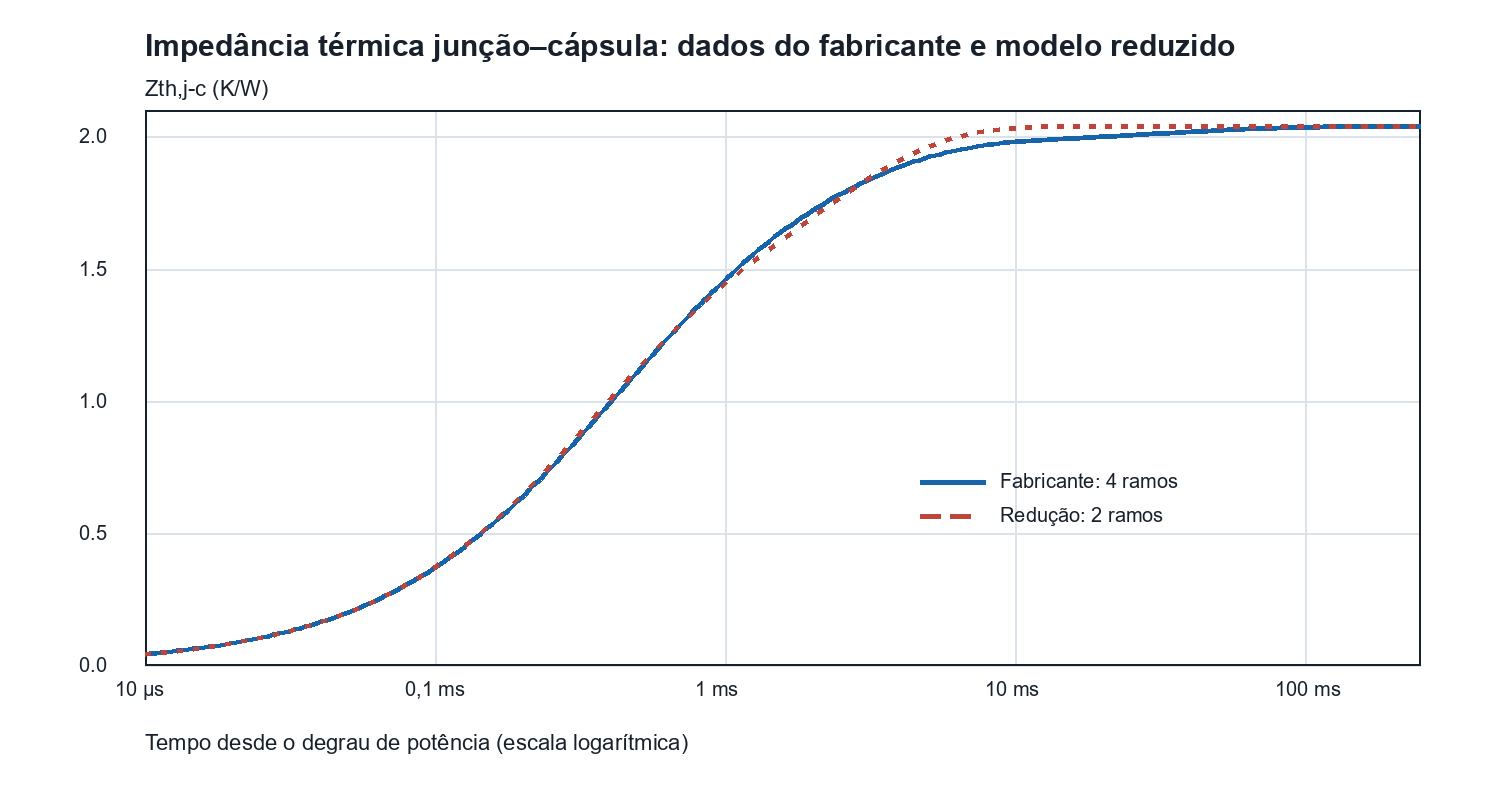
\includegraphics[width=.96\linewidth]{figuras/ajuste_impedancia.png}
\caption{Comparação calculada da impedância transitória. Não são dados VHIL.}
\end{figure}

\section{Formulação e análise dinâmica}
Cada ramo satisfaz conservação de energia em uma capacitância térmica
equivalente:
\begin{equation}
 C_i\dot\theta_i=P-\theta_i/R_i,\qquad
 \dot\theta_i=-\theta_i/\tau_i+(R_i/\tau_i)P,\quad i=1,2.
\end{equation}
Aqui $C_i$ em J/K, $\dot\theta_i$ em K/s, $P$ e $\theta_i/R_i$ em W.
Com $x=[\theta_1\;\theta_2]^T$ e $y=T_j-T_c$,
\begin{equation}
 \dot x=\underbrace{\begin{bmatrix}-1/\tau_1&0\\0&-1/\tau_2\end{bmatrix}}_{A}x+
 \underbrace{\begin{bmatrix}R_1/\tau_1\\R_2/\tau_2\end{bmatrix}}_{B}P,
 \qquad y=\begin{bmatrix}1&1\end{bmatrix}x.
\end{equation}
Consequentemente, $G(s)=\Delta T_j(s)/P(s)=R_1/(1+\tau_1s)+
R_2/(1+\tau_2s)$. Os polos, iguais aos autovalores de $A$, são
$-3473{,}762$ e $-494{,}766$ s$^{-1}$. As constantes de tempo são
$0{,}287872$ e $2{,}021157$ ms. A razão entre escalas é $7{,}02$;
o passo de $10\,\mu$s resolve a constante rápida com aproximadamente
29 amostras. Usando o denominador de segunda ordem,
$\omega_n=1/\sqrt{\tau_1\tau_2}=1310{,}992$ rad/s e
$\zeta=(\tau_1+\tau_2)/(2\sqrt{\tau_1\tau_2})=1{,}514>1$.
Portanto, a resposta é superamortecida, sem frequência amortecida real
nem sobressinal intrínseco. A aproximação conservadora $4\tau_2$ dá
$8{,}085$ ms para a acomodação a $2\%$; a curva composta pode atingir a
banda antes desse limite.

Para $P=10$ W e $x(0)=0$, a solução de referência é
$T_j(t)=25+10\sum_iR_i(1-e^{-t/\tau_i})$ em $^\circ$C e o equilíbrio
do modelo é $45{,}39707\,^\circ$C. Na relaxação com
$x_i(0)=10R_i$ e $P=0$, tem-se
$T_j(t)=25+10\sum_iR_i e^{-t/\tau_i}$.
O pulso de 10 W por 10 ms é obtido por superposição de dois degraus.

\section{Implementação e ensaios}
No Schematic Editor, o arquivo \texttt{Equipe04\_TermicoRC\_IGBT.tse}
contém um sequenciador e três cópias independentes do mesmo RC: degrau
a partir de zero, relaxação a partir do equilíbrio e pulso. Em cada
período de $0{,}1$ s, o sinal de \texttt{reset\_ciclo} reinicializa os
estados; o degrau liga de 10 a 60 ms, e o pulso de 10 a 20 ms. Em cada
atualização, o código usa a solução exata para entrada constante no
intervalo de amostragem:
\begin{equation}
 \theta_i[k+1]=\theta_i[k]+(1-e^{-T_s/\tau_i})
 \big(R_iP[k]-\theta_i[k]\big),\quad T_s=10\,\mu\mathrm{s}.
\end{equation}
Os seis probes incluem duas potências, três temperaturas e o reset. A
captura programática pelo recurso \emph{Capture} deve usar passo de
$10\,\mu$s e guardar $30\,000$ amostras, sem substituição por
leitura ponto a ponto. O arquivo \texttt{capturar\_vhil.py} compila,
carrega em Virtual HIL e salva CSV, metadados e hashes; o script
\texttt{analisar\_captura.py} só produz métricas experimentais se o
CSV e o hash do .tse conferirem.

\clearpage
\begin{figure}[ht!]
\centering
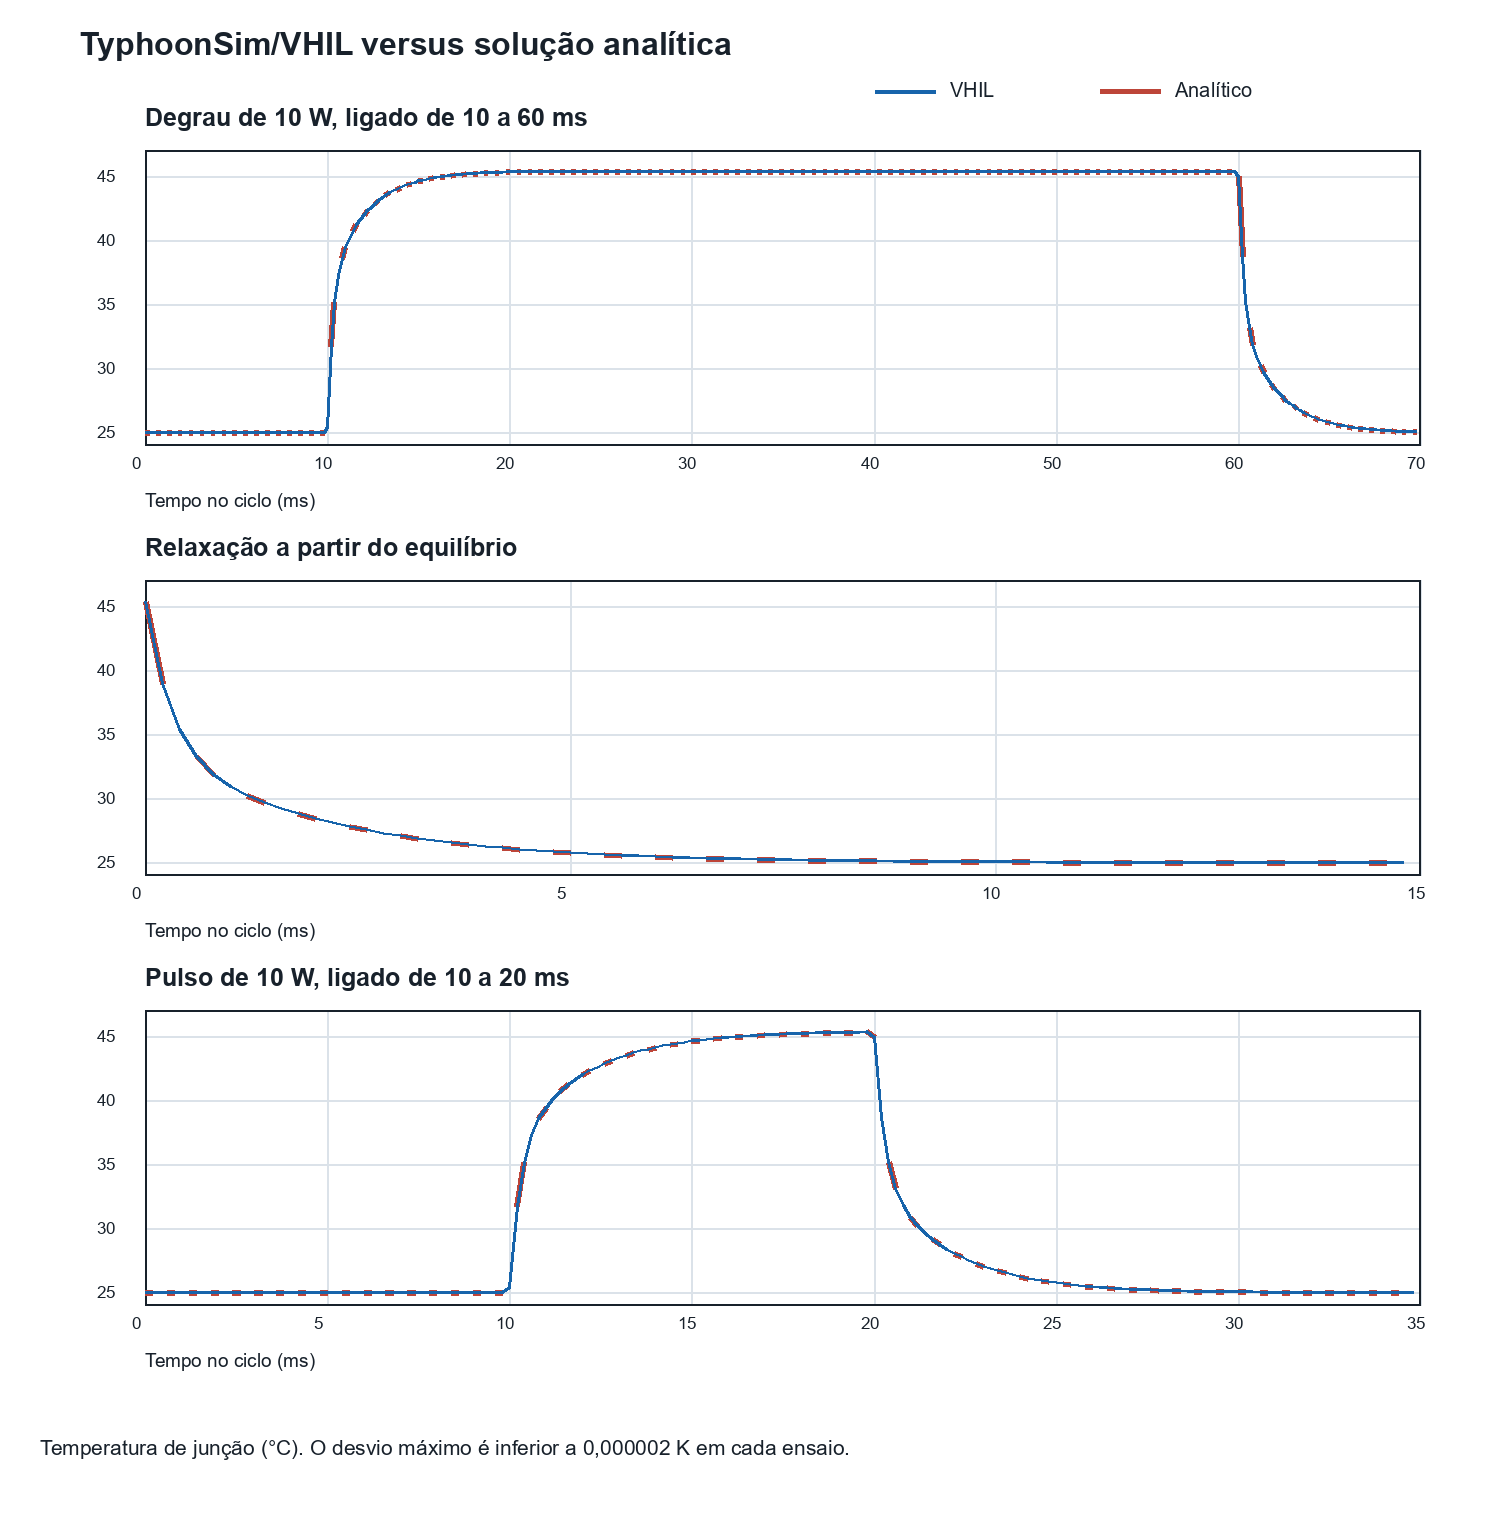
\includegraphics[width=.96\linewidth]{figuras/ensaios_vhil.png}
\caption{Resultados efetivamente capturados no TyphoonSim (azul) e
soluções analíticas (vermelho tracejado) nos três ensaios. As curvas
praticamente coincidem; a escala vertical é de dezenas de graus, enquanto
o erro máximo é da ordem de $10^{-6}$~K.}
\end{figure}
\clearpage

\section{Verificação, precisão e resultado experimental}
A atualização exata ZOH coincide com a solução analítica do degrau com
erro máximo de $2{,}1\times10^{-13}$ K em dupla precisão. Uma integração
RK4 independente com passo de $1\,\mu$s apresentou erro máximo de
$5{,}0\times10^{-12}$ K nos pontos verificados. Em cálculo de referência
com estados float32, o desvio máximo frente a float64 foi
$1{,}10\times10^{-4}$ K. Esses testes são externos ao TyphoonSim e
verificam a discretização e a solução, não a execução da implementação.

\noindent\textbf{Execução em Virtual HIL.} O arquivo .tse compilou com
sucesso no Typhoon HIL Control Center 2026.2; o log informa seis probes,
um núcleo de processamento padrão em uso e restrições de tempo atendidas.
A simulação usou passo-base de $0{,}2\,\mu$s. A API \emph{Capture} aplicou
decimação 50, produzindo 30.000 amostras a $10\,\mu$s, com três pulsos de
reinício. O ciclo analisado inicia na amostra 7073 do CSV. A integridade
do CSV, do modelo .tse e do .cpd foi conferida por SHA-256 com os
metadados da captura. As potências capturadas reproduzem o degrau de
10 a 60 ms e o pulso de 10 a 20 ms em cada ciclo de 100 ms.

\begin{center}\begin{tabular}{lr}\toprule
Medida VHIL & Valor \\ \midrule
Maior erro, degrau & $1{,}907\times10^{-6}\,\mathrm{K}$ \\ 
Maior erro, relaxa\c{c}\~ao & $1{,}895\times10^{-6}\,\mathrm{K}$ \\ 
Maior erro, pulso & $1{,}906\times10^{-6}\,\mathrm{K}$ \\ 
Subida 10--90\% & $3{,}0003$~ms \\ 
Atingimento de 98\% & $6{,}3038$~ms \\ 
\bottomrule\end{tabular}
\end{center}
Em cada ensaio o erro máximo é inferior a $1{,}91\,\mu$K, e o pico do
degrau foi $45{,}3970718384\,^\circ$C, frente ao equilíbrio teórico de
$45{,}39707\,^\circ$C. O critério de erro máximo de $0{,}15$ K foi
satisfeito. A concordância verifica a implementação numérica,
\emph{não} a física do IGBT: VHIL e solução analítica empregam o
mesmo modelo.

\section{Limitações e conclusão}
O modelo trata só o caminho térmico junção--cápsula do IGBT, não
temperatura ambiente, dissipador, perdas elétricas dependentes da
temperatura ou o diodo integrado. Um valor constante de $T_c$ é uma
condição de contorno, não uma previsão para um dispositivo real sem
refrigeração. O ajuste de segunda ordem preserva o ganho estacionário
da curva de quatro ramos e apresenta erro relativo máximo de $2{,}679\%$
na faixa estudada; fora dela, a extrapolação não foi validada. A análise
teórica, numérica e a captura em Virtual HIL documentam a caracterização
pedida no Banco e no Guia. A correspondência com o fabricante é limitada
à aproximação da curva publicada; não houve ensaio térmico em hardware
físico nem validação do modelo fora da faixa declarada.

\begin{thebibliography}{9}
\bibitem{banco} ECOM060. \emph{Banco de Sistemas -- corrigido 01}, 2026.2,
especialmente Sistema 6 e requisitos de ficha/verificação.
\bibitem{guia} ECOM060. \emph{Guia de Caracterização}, 2026.2.
\bibitem{infineon} Infineon Technologies. \emph{IKD04N60RF Datasheet},
versão 2.6, Fig.~21 e tabela térmica.
\href{https://www.infineon.com/dgdl/Infineon-IKD04N60RF-DS-v02_06-EN.pdf?fileId=db3a30433c5c92fb013c5d6c806d00dc}{PDF oficial}.
\bibitem{foster} Infineon Technologies. \emph{IGBT Modules: Explanation of
Technical Information}, AN2011-05.
\href{https://www.infineon.com/dgdl/Infineon-AN2011_05_IGBT_Modules_Explanation-ApplicationNotes-v01_02-EN.pdf?fileId=db3a304334c41e910134eb12584604e2}{PDF oficial}.
\end{thebibliography}
\end{document}
